\documentclass[useAMS,usenatbib,referee]{biom}

\usepackage{amsmath}
\usepackage[figuresright]{rotating}

\graphicspath{{include/}}

\def\bSig\mathbf{\Sigma}
\newcommand{\VS}{V\&S}
\newcommand{\tr}{\mbox{tr}}



\title{Empirical Bayes analysis for detection of gene heterosis in RNAseq data}

\author{Jarad Niemi$^*$\email{niemi@iastate.edu}, 
Eric Mittman, 
Will Landau, and 
Dan Nettleton \\
Department of Statistics, Iowa State University, Ames, Iowa, U.S.A.}

\begin{document}

\date{{\it Received December} 2014} 

\pagerange{\pageref{firstpage}--\pageref{lastpage}} 
\volume{VV}
\pubyear{YYYY}
\artmonth{MM}
\doi{x}

\label{firstpage}

\begin{abstract}
Heterosis, or hybrid vigor, refers to the enhancements in the phenotype of hybrid progeny relative to their inbred parents. Although the heterosis phenomenon is extensively utilized in agriculture, the molecular basis is still unknown. In an effort to understand phenotypic heterosis at the molecular level, researchers have begun to compare expression levels of thousands of genes between parental inbred lines and their hybrid offspring to search for evidence of gene expression heterosis in RNA sequencing (RNAseq) experiments. Standard statistical approaches for RNAseq experiments struggle with the composite null hypothesis in gene heterosis testing. To address these shortcomings, we develop a hierarchical model based on a negative-binomial data model and a computationally tractable empirical Bayes approach. We demonstrate improvements over alternative methods via a simulation study based on a maize experiment and then analyze that maize experiment. This article has supplementary material online.
\end{abstract}

\begin{keywords}
Empirical Bayes; Gene expression; Heterosis; Hierarchical model; Negative binomial; RNAseq.
\end{keywords}

\maketitle

%  A maximum of six (6) tables or figures combined is often required.''

\section{Introduction}
\label{s:intro}

% Need to udpate as this is directly from Tieming's paper
Heterosis, or hybrid vigor, refers to the enhancements in the phenotype of hybrid progeny relative to their inbred parents. Taking maize as an example, the offspring from crossing the inbred lines B73 and Mo17 grow taller, mature faster, and produce greater yields than their parent lines \citep{hallauer1981quantitative, hallauer2010quantitative}. Ever since heterosis was scientifically documented by \cite{darwin1876effects}, it has been successfully manipulated to improve many species for the food, feed, and fuel industries, such as rice \citep{yu1997importance}, alfalfa \citep{riday2002heterosis}, tomatoes \citep{krieger2010flowering}, and fish \citep{wohlfarth1993heterosis}. Despite the intensive study and successful utilization of heterosis, the basic genomic mechanisms remain unclear \citep{coors1999genetics, lippman2007heterosis}. Researchers speculate that gene-expression heterosis $-$ i.e, enhanced expression of one or more genes in the hybrid relative to the inbred parents $-$ is a possible  mechanisms for the phenotypic heterosis \citep{swanson2006all, springer2007allelic}.

Recently, \cite{ji2014estimation} introduced an approach to assess gene heterosis using microarray data under the assumption that these data are continuous. They built a normal hierarchical model for gene expression that allows borrowing of information across genes for means and variances. They introduced an empirical Bayes framework that first estimates model hyperparameters, then estimates the posterior distribution for gene-specific parameters conditional on those hyperparameters, and finally computes heterosis probabilities based on integrals of regions under this posterior. This development was necessary due to the composite null hypothesis in tests for heterosis. These hypotheses, which many available methods do not fully accommodate, remain a challenge in the transition from continuous data to count data. Building on the work of \citeauthor{ji2014estimation} with the normal data model, we construct a hierarchical model based on a negative-binomial data model. We also utilize an empirical Bayes approach to obtain \emph{maximum a posterior} (MAP) estimates of the hyperparameters and the posterior distributions for the gene-specific parameters conditional on those hyperparameters. 

The remainder of the paper proceeds as follows. Section \ref{s:method} presents the proposed hierarchical model, an empirical Bayes method of estimating the parameters, and the calculation of posterior probabilities of gene heterosis. Section \ref{s:simulation} presents a simulation study based on a maize experiment and compares our approach to alternative methods. Section \ref{s:maize} analyzes a maize experiment where phenotypic heterosis is well established and identifies genes demonstrating heterosis. The data and code necessary to perform this analysis is available in the Supplemental Material. Section \ref{s:discussion} summarizes the work and suggests directions for future research.


\section{Empirical Bayes identification of gene heterosis from RNAseq counts}
\label{s:method}

An RNA sequencing (RNAseq) experiment to identify genes demonstrating heterosis consists of three genetic varieties: two parental varieties (P1 and P2) and a cross between these two varieties called the hybrid (H). For each variety, replicate RNA samples are isolated and assessed for quality. cDNA libraries, or collections of short cDNA fragments, are constructed. Then, next generation sequencing technology is used to determine the \emph{reads}, or nucleotide sequences, in the cDNA libraries. These reads are processed using bioinformatic algorithms to match the reads to genes, or specific gene transcripts, exons, microRNAs, etc. The result of matching reads to features are summarized by a gene $\times$ sample matrix of counts. See \cite{nettleton2014design} for more details on RNAseq experiments, and see \cite{paschold2012complementation} for the biological background behind the above steps.

To use RNAseq counts to identify genes displaying heterosis, we build a hierarchical model to borrow information on gene-variety means and gene-specific overdispersion parameters, estimate the parameters using a empirical Bayes procedure implemented in the statistical software {\tt Stan}, and calculate empirical Bayes posterior probabilities for heterosis. 


\subsection{Hierarchical model for RNAseq counts}
\label{s:model}

Let $Y_{gvi}$ be the count for gene $g=1,\ldots,G$, variety $v=1,\ldots,V$, and replicate $i=1,\ldots,n_v$. As shown in equation \eqref{e:data}, we assume a negative binomial for the counts with a mean that depends on the gene-variety combination through $\mu_{gv}$ and the sequencing depth $\gamma_{vi}$ and a gene-specific overdispersion $\psi_g$. 
\begin{equation} 
Y_{gvi} \stackrel{ind}{\sim} NB(e^{\mu_{gv}+\gamma_{vi}},\psi_g) 
\label{e:data}
\end{equation}
where $NB(\eta,\psi)$ indicates a negative-binomial with expectation $\eta$ and variance $\eta+\psi\eta^2$, and $ind$ indicates the observations are conditionally independent.

We present a hierarchical model for the sequencing depth, overdispersion, and gene-variety parameters. The sample-specific sequencing depth terms are assumed to follow a normal distribution, i.e. $\gamma_{vi} \stackrel{ind}{\sim} N(0,\tau_\gamma^2)$. (These terms are the normalization factors that practitioners typically estimate for each sample and then treat as constant in further analysis.) The logarithm of the gene-specific overdispersion parameters and the gene-specific variety effects are assumed to have a joint normal distribution, i.e. 
$\theta_g = [\mu_g, \log(\psi_g)]^\top \stackrel{ind}{\sim} N\left(\eta, \Sigma\right)$
where $\mu_g = (\mu_{g1},\ldots,\mu_{gV})'$. We consider an \emph{independent} model in which $\Sigma$ is diagonal with elements $\sigma_1^2,\ldots,\sigma_{V+1}^2$ and a \emph{covariance} model in which we estimate all parameters in $\Sigma$.

We assume improper uniform priors for $\eta$ and take $\tau_\gamma\stackrel{ind}{\sim} Ca^+(0,3)$, where 0 and 3 are the location and scale parameters, respectively, of the untruncated half-Cauchy distribution. In the independent model, we also assign the $Ca^+(0,3)$ prior to the diagonal elements of $\Sigma$. In the covariance model, we assume a conjugate, proper inverse Wishart distribution with degrees of freedom $V+2$ and an identity scale matrix, resulting in marginally uniform correlations. 

\subsection{Empirical Bayes}
\label{s:ebayes}

We separate the parameters of the model in Section \ref{s:model} into gene-specific parameters $\theta = (\theta_1,\ldots,\theta_G)$ and hyperparameters $\pi = (\gamma,\eta, \Sigma)$, where $\gamma = (\gamma_{11},\ldots,\gamma_{Vn_V})$. We employ an optimization procedure to obtain the \emph{maximum a posteriori} (MAP) estimate for $\pi$, denoted $\hat{\pi}$, and then base gene-specific inference on the posterior conditional of this estimated hyperparameter. Conditional on the hyperparameters, the gene-specific parameters are independent as in equation \eqref{e:condind}. Thus, conditional posterior inference for the gene-specific parameters can be obtained independently and in parallel.
\begin{align}
p\left(\theta\left|y,\hat{\pi}\right.\right) 
%&= \prod_{g=1}^G p\left(\theta_g\left|y_g,\hat{\pi}\right.\right) = \prod_{g=1}^G p\left(y_g\left|\theta_g,\hat{\gamma}\right.\right) p\left(\theta_g\left|\hat{\pi}\right.\right) \nonumber \\
&\propto \prod_{g=1}^G \left[ \prod_{v=1}^V \prod_{i=1}^{n_v} NB\left(y_{gvi}\left|e^{\mu_{gv}+\hat{\gamma}_{vi}},\psi_g\right.\right) \right] N\left(\left.\left[\mu_g, \log(\psi_g) \right]^\top\right|\hat{\eta}, \hat{\Sigma} \right) 
\label{e:condind}
\end{align}


To perform the optimization, we use the statistical software, {\tt Stan} \citep{stan-software:2014}, executed through the RStan interface \citep{rstan-software:2014} in R \citep{R2014}. The Stan software allows the construction of general Bayesian models with the primary restriction that all unknown parameters are continuous. With a fully constructed model, the software can obtain MAP estimates \cite[Section 50.3,][]{stan-manual:2014} using the {\tt optimizing} function in RStan. It was necessary to use the L-BFGS algorithm \cite[Section 55,][]{stan-manual:2014} and reasonable starting values obtained via {\tt edgeR}, presumably due to the large dimension of the optimization. The {\tt Stan} software also includes the RStan function, {\tt sampling}, an implementation of a Markov chain Monte Carlo (MCMC) algorithm for obtaining samples from the posterior. By default, Stan uses a no-U-turn sampler \citep{hoffman2013no}, a variant of Hamiltonion Monte Carlo \citep{neal2011mcmc}.

As we have not integrated out the gene-specific parameters when obtaining the MAP estimate, we actually receive a joint MAP estimate of $\theta$ and $\pi$. We explicitly use the MAP estimate of $\pi$ when obtaining empirical Bayes posterior samples for the gene-specific parameters as in equation \eqref{e:condind}. The MAP estimate of $\theta$ can also be used in this step as initial values for the MCMC. 

\subsection{Gene heterosis}
\label{s:gene_heterosis}

As defined in Section \ref{s:intro}, heterosis is increased (or decreased) phenotypic expression in a hybrid relative to its inbred parents. Thus, when attempting to identify heterosis, there are $V=3$ varieties of interest. We let $v=1,2$ be the two parental varieties and $v=3$ be the hybrid. We define gene heterosis to be the differential expression of a gene in the hybrid relative to its parents. For a specific gene $g$, low-parent gene heteorisis (LPH) occurs when $\mu_{g3}< \min(\mu_{g1},\mu_{g2})$ 
%, mid-parent gene heterosis occurs when $\mu_{g1}\le \mu_{g3}\le \mu_{g2}$ if $\mu_{g1}\le \mu_{g2}$ (or $\mu_{g1}\ge \mu_{g3}\ge \mu_{g2}$ if $\mu_{g1}\ge \mu_{g2}$), 
and high-parent gene heterosis (HPH) occurs when $\max(\mu_{g1},\mu_{g2}) < \mu_{g3}$. For simplicity, we define \emph{extreme gene heterosis} (EH) to be the event of LPH or HPH. Equation \eqref{e:hypotheses} shows the most important hypotheses, where $H_0$ indicates no EH and $H_1$ indicates EH. 
\begin{align}
H_{g0}:&\mu_{g1}\le \mu_{g3}\le \mu_{g2} \mbox{ or } \mu_{g1}\ge \mu_{g3}\ge \mu_{g2} \mbox{\ \ vs.\ \ } \nonumber \\
H_{g1}:&\mu_{g3}< \min(\mu_{g1},\mu_{g2}) \mbox{ or } \max(\mu_{g1},\mu_{g2}) < \mu_{g3}.
\label{e:hypotheses}
\end{align}
We evaluate these hypotheses based on empirical Bayes estimates of their posterior probabilities, e.g. 
\begin{align}
P\left(H_{g1}|y, \hat{\pi}_{MAP}\right) &= P\left(\left.\mu_{g3}< \min(\mu_{g1},\mu_{g2}) \mbox{ or } \max(\mu_{g1},\mu_{g2}) < \mu_{g3}\right| y, \hat{\pi}_{MAP}\right) \nonumber \\
&\approx \frac{1}{M} \sum_{m=1}^M \mathrm{I}\left(\mu_{g3}^{(m)}< \min\left(\mu_{g1}^{(m)},\mu_{g2}^{(m)}\right) \mbox{ or } \max\left(\mu_{g1}^{(m)},\mu_{g2}^{(m)}\right) < \mu_{g3}^{(m)}\right) \label{e:probs}
\end{align}
where $\mu_g^{(m)} = \left(\mu_{g1}^{(m)},\mu_{g2}^{(m)},\mu_{g3}^{(m)}\right)$ is the $m^{th}$ MCMC sample from the empirical Bayes posterior, and $\mathrm{I}(A)$ is 1 if A is true and 0 otherwise. The set of probabilities $P\left(H_{g1}|y, \hat{\pi}_{MAP}\right)$ for $g=1,\ldots,G$ can be used to provide a list of genes sorted by the relative strength of evidence of extreme heterosis. Geneticists can use this list to prioritize future experiments to understand the genetic mechanism for heterosis.  

\section{Simulation study based on maize experiment}
\label{s:simulation}

% \subsection{Coverage for our model}
% \input{../temp/analyze-heterosis/FIGURES/coverage}

To assess the efficacy of our method to identify genes demonstrating heterosis, we used a maize data set with parental varieties B73 and Mo17 and the hybrid variety (B73 $\times$ Mo17) \citep{paschold2012complementation}. Section \ref{s:maize} describes this dataset in detail. We compared our method to approaches using the R packages {\tt edgeR}, {\tt baySeq}, and {\tt ShrinkBayes}.

\subsection{Constructing simulated data}
\label{s:sim_data}

Initially, the maize experiment had RNAseq counts for 39,656 genes and 4 replicates per variety. We eliminated low count genes by removing any gene with three or more zeros for any variety and genes whose mean count across the varieties was less than one, resulting in 27,888 remaining genes.

Next, we applied the {\tt edgeR} package \citep{robinson2010edgeR} from Bioconductor \citep{gentleman2004bioconductor} to the maize data to obtain sample-specific normalization factors, then gene-specific dispersions, and finally gene-variety-specific location parameters. We treated these parameters as the truth for the simulation study: i.e. a gene with $\mu_{g3} < \min(\mu_{g1}, \mu_{g2})$ was considered to have LPH, while a gene with $\max(\mu_{g1},\mu_{g2}) < \mu_{g3}$ was considered to have HPH. This technique ensured that our simulated datasets maintained the existing covariance structure among the gene-variety means of the original maize data.

Using these parameters and normalization factors, we simulated data according to the negative-binomial model in equation \eqref{e:data} independently for each gene. For each simulation, low count genes $-$ those with three or more zeros in any variety or whose mean count across the varieties was less than one $-$ were removed. We retained a random subset of 25,000 genes from those with high enough counts. We repeated this simulation process 10 times for each of 4, 8, and 16 replicates per variety, reusing normalization factors when necessary.

\subsection{Alternative methods}
\label{s:alternative}

Existing RNAseq data analysis methods are not specifically designed to identify gene heterosis, but we adapted the approaches in {\tt edgeR}, {\tt baySeq}, and {\tt ShrinkBayes} to provide a measure of the strength of extreme heterosis for each gene such that large values of this measure indicate support for extreme heterosis.

The {\tt edgeR} approach is designed to apply a negative-binomial log-linear model to test for differential expression between any two varieties \citep{robinson2007moderated, robinson2010edgeR}. To construct a measure of heterosis, we computed the maximum likelihood estimates of the mean expression effects of all genes using {\tt edgeR}'s built-in Fisher scoring algorithm, and then used the likelihood ratio test functionality to calculate two legitimate p-values for each gene: one for the null hypothesis that the hybrid's mean expression is the same as that of parent 1 and the second for the analogous test involving parent 2. For each gene, if the estimated mean expression level of the hybrid is between the estimated mean expression levels of the parents, we set the measure of heterosis to zero. Otherwise, we set the measure of heterosis to be one minus the p-value corresponding to the parent with estimated expression level closer to that of the hybrid. 

The {\tt baySeq} approach \citep{hardcastle2010bayseq, hardcastle2012baySeq} allows for a wider range of hypotheses for each gene, including $H_1: \mu_{g1}=\mu_{g2}=\mu_{g3}$, $H_2: \mu_{g1}=\mu_{g2}$, $H_3: \mu_{g1}=\mu_{g3}$, $H_4: \mu_{g2}=\mu_{g3}$, and $H_5:$ all $\mu_g$'s are distinct. In a technique similar to our application of {\tt edgeR}, we used the posterior probabilities of these hypotheses to construct a measure of heterosis for each gene. We set this measure to zero if the hybrid's maximum likelihood estimate of the mean expression level calculated using {\tt edgeR} is between those of the parents. Otherwise, the measure is the sum of the posterior probabilities of $H_2$ and $H_5$, the only hypotheses that allow for extreme heterosis.

The {\tt ShrinkBayes} package implements fully Bayesian inference through integrated nested Laplace approximation (INLA) \citep{rue2009approximate,van2014shrinkbayes}. A limitation of INLA is that it only provides approximations to marginal posteriors for parameters or linear combinations of parameters rather than an approximation to the full posterior. Thus, we cannot directly estimate nonlinear quantities such as $P(\mu_{g3} < \min(\mu_{g1},\mu_{g2})|y)$. To circumvent this limitation, we reparameterized the independence model in Section \ref{s:model} using the approach in \cite{ji2014estimation}. 
Let $\phi_g = (\mu_{g1}+\mu_{g2})/2$ be the parental log-mean, $\alpha_g = (\mu_{g2}-\mu_{g1})/2$ be the half parental difference, and $\delta_g = \mu_{g3} - \phi_g$ be the hybrid effect. After fitting the model with {\tt ShrinkBayes}, we constructed a measure of heterosis for each gene. For gene $g$, we used the estimated posterior means $\hat{\delta}_g$ and $\hat{\alpha}_g$ of $\delta_g$ and $\alpha_g$, respectively, along with appropriate posterior probabilities. Specifically, the measure of heterosis for gene $g$ is zero if $|\hat{\delta}_g| \le |\hat{\alpha}_g|$, $P(\delta_g + \alpha_g > 0 |y)$ if $\hat{\delta}_g > -\hat{\alpha}_g \ge 0$, $P(\delta_g - \alpha_g > 0 |y)$ if $\hat{\delta}_g > \hat{\alpha}_g \ge 0$, $P(\delta_g - \alpha_g < 0 |y)$ if $\hat{\delta}_g < \hat{\alpha}_g \le 0$, and $P(\delta_g + \alpha_g < 0 |y)$ if $\hat{\delta}_g < -\hat{\alpha}_g \le 0$.  

\subsection{Results}

For each of the methods above, as well as the method described in Section \ref{s:gene_heterosis}, we sorted genes according to the plausibility of heterosis. From these sorted lists, we constructed receiver-operating characteristic (ROC) curves to evaluate the ability of these methods to identify genes with heterosis, as defined in Section \ref{s:sim_data}  \citep{landau2013dispersion}. A representative set of ROC curves is shown in Figure \ref{f:roc}. 
\begin{figure}[htbp]
\centerline{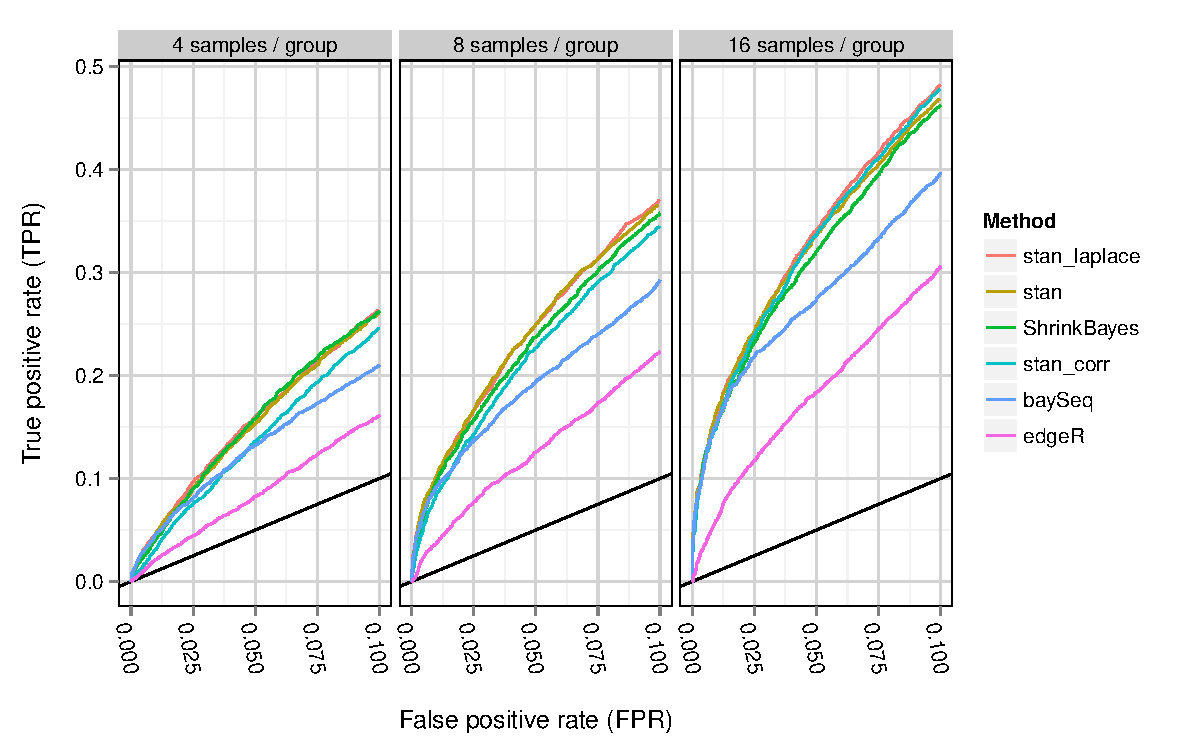
\includegraphics[width=\textwidth]{exampleROC0_1}}
\caption{Repersentative ROC curves for false positive rates below 0.1 for the approaches using {\tt edgeR}, {\tt baySeq},  and {\tt ShrinkBayes} described in Section \ref{s:alternative}, along with the independent and covariance methods using {\tt RStan} described in Section \ref{s:gene_heterosis}.}
\label{f:roc}
\end{figure}
For this simulation, we can see that the approaches based on the model in Section \ref{s:model} $-$ i.e. both RStan approaches and the ShrinkBayes approach $-$ provide the best true positive rate for a given false positive rate. Also, as expected, as the sample size increases, our ability to distinguish genes with heterosis from genes without improves.

Figure \ref{f:auc} provides the area under the ROC curve below a false positive rate of 0.1 across the 10 simulations for each of the 3 different sample sizes. 
\begin{figure}
\centerline{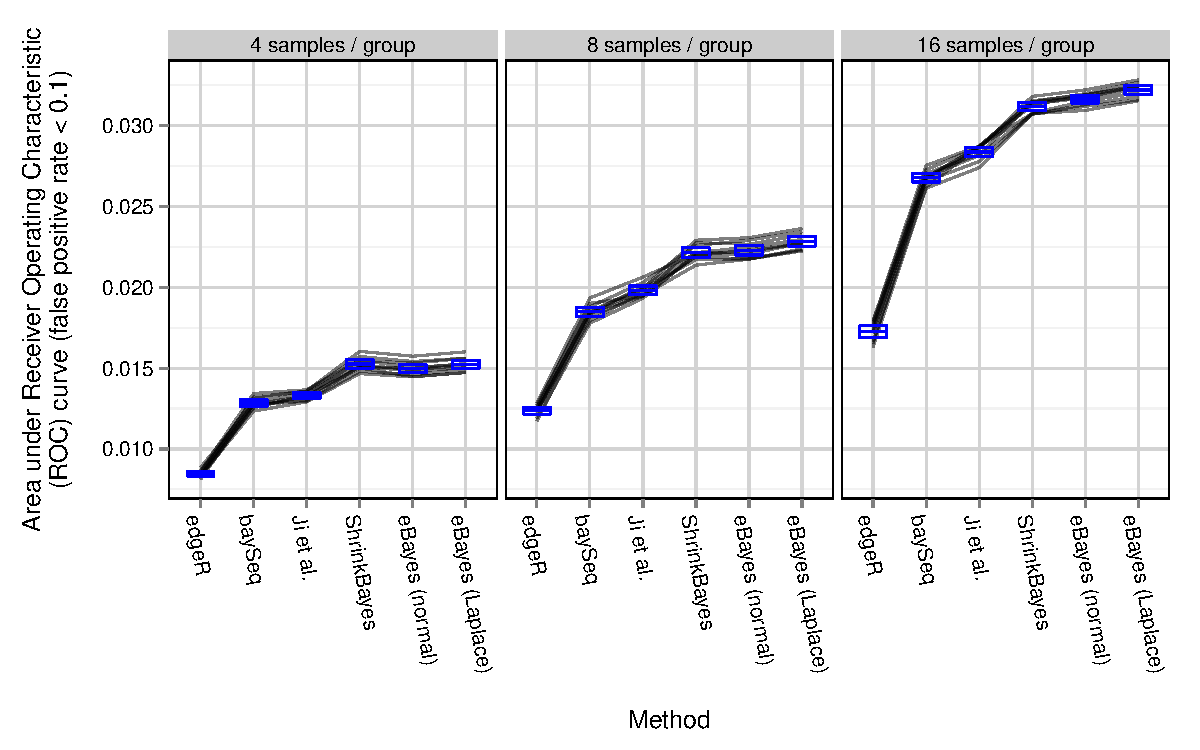
\includegraphics[width=\textwidth]{auc-facet-TRUE}}
\caption{Area under the ROC curves below a false positive rate of 0.1 for 3 different sample sizes for the approaches using {\tt edgeR}, {\tt baySeq},  and {\tt ShrinkBayes} described in Section \ref{s:alternative} , along with the independent and covariance methods using {\tt RStan} described in Section \ref{s:gene_heterosis}. Each line is a different simulation while the blue box indicates mean AUC and its standard error across the simulations.}
\label{f:auc}
\end{figure}
The pattern appears to hold, with the {\tt RStan} and {\tt ShrinkBayes} techniques outperforming the other two. While there does not appear to be a significant difference between {\tt ShrinkBayes} and the independence model using {\tt RStan}, performance appears to decrease for the model where a covariance is estimated, at least for smaller sample sizes.


\section{Heterosis in maize experiment}
\label{s:maize}

We used our method to analyze a maize data set on gene expression in parental lines B73 and Mo17 and the hybrid genotype (B73$\times$Mo17). The data are available in the Supplemental Materials. Each variety had four biological replicates measured with Illumina methodology and equipment. Reads were mapped to the whole reference genome using the short reads aligner, NOVOALIGN. For more specifics, please see \cite{paschold2012complementation}. 

A total of 39,656 genes among $V=3$ varieties, each with $n_v=4$ replicates, were available for analysis. As before, we eliminated genes with three or more zeros for any variety and genes with mean expression less than one across all samples, resulting in a total of $G=27,888$ genes present in the analysis. 

We found MAP estimates for both the independence and covariance models as shown in Table \ref{t:map}. 
% Need MAP estimates table and discussion

Independently for each gene, we ran an MCMC conditional on the hyperparameters to obtain empirical Bayes posterior distributions for all gene-specific parameters. Each MCMC was run using 4 chains with initial values randomly drawn by {\tt Stan}. Each chain ran for a total of 2000 iterations, with 1000 iterations of burn-in and the remaining 1000 draws thinned by a factor of 4 for storage reasons. The potential scale reduction factor, $\hat{R}$, was computed for each parameter \citep{Gelm:Rubi:infe:1992, Broo:Gelm:gene:1997}. If the maximum value of $\hat{R}$ was larger than 1.1, the total length was increased by 500, with the burn-in increased proportionally, and the chain was rerun. This process was repeated until the maximum $\hat{R}$ was less than 1.1 for all parameters.

With posteriors for all parameters, we can calculate empirical Bayes posterior probabilities for LPH and HPH. For each gene, the quantity of interest is likely to be the maximum of these two probabilities. For each gene with a high probability of either HPH or LPH, the magnitude of the effect is of interest. Thus, we calculate estimated effect sizes using the estimated posterior means of the gene-specific parameters using the formula 
\begin{equation}
\mbox{estimated effect size} = \left\{ 
\begin{array}{ll}
\hat{\mu}_{g3} - \min(\hat{\mu}_{g1},\hat{\mu}_{g2}) & \mbox{if } \hat{\mu}_{g3} < \min(\hat{\mu}_{g1},\hat{\mu}_{g2}) \\
\hat{\mu}_{g3} - \max(\hat{\mu}_{g1},\hat{\mu}_{g2}) & \mbox{if } \hat{\mu}_{g3} > \max(\hat{\mu}_{g1},\hat{\mu}_{g2}) \\
0 & \mbox{otherwise}.
\end{array} 
\right. 
\label{e:effect_size}
\end{equation}

Figure \ref{f:volcano} provides a volcano plot to visualize the maximum of the probabilities of LPH and HPH versus estimated effect size. The figure shows a line at zero for probabilities less than 0.5 because the effect size is set to 0 for the vast majority of genes. Above a probability of 0.5, we see a prototypical volcano pattern, with increased extreme heterosis probability corresponding to larger estimated effect sizes and no estimated effect sizes near zero for genes with high extreme heterosis probability. We also see asymmetry, with larger negative effect sizes than positive effect sizes, because many genes have hybrid counts near zero and relatively high parental counts. Genes with high probabilities of extreme heterosis and large estimated effect sizes are candidates for further investigation.

% Compare independence and volcano plots

\begin{figure}
\centerline{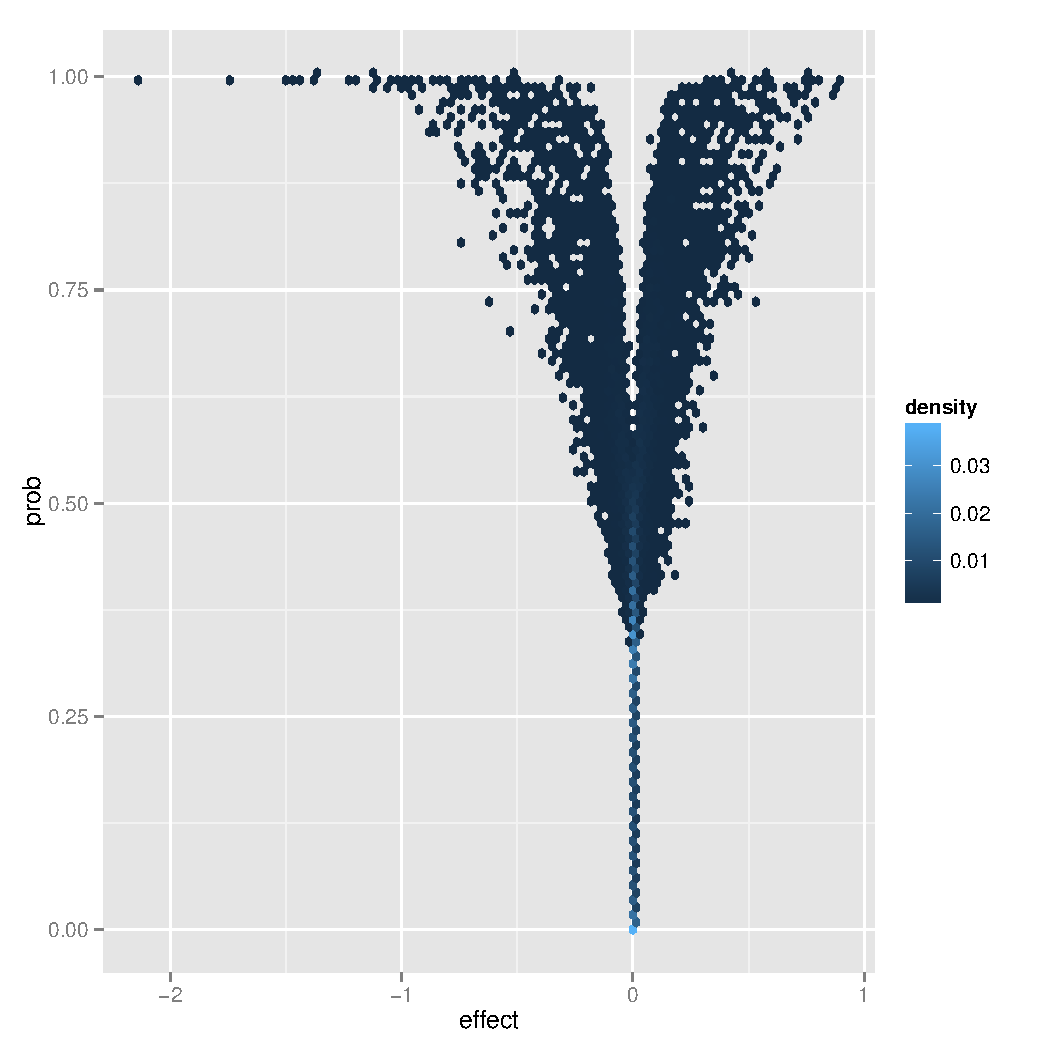
\includegraphics[width=\textwidth]{volcano}}
\caption{A two-dimensional histogram of the maximum of the LPH and HPH probabilities versus estimated effect size defined in equation \ref{e:effect_size} for the B73 $\times$ Mo17 maize experiment using the independence model.}
\label{f:volcano}
\end{figure}

With almost 30,000 genes in our data set, we can evaluate the normality assumption for the gene-specific parameters. Figure \ref{f:normality} provides histograms of components of $\theta$ from a single MCMC iteration. If the prior assumption of normality is correct, we would expect these histograms to show approximate normality. The marginal histograms show a bimodal distribution for $\mu$ with a secondary peak around relatively small values. The bivariate histograms amongst the components of $\mu$ show a high correlation but with a heavy-tail toward small values of both components of $\mu$. With stricter gene-inclusion criterion, it is possible both the secondary peak and the heavy-tailedness could be eliminated. The histogram for $\log(\psi)$ displays a heavy-tail to the right and the bivariate histograms show a pattern of near independence between $\log(\psi)$ and $\mu_g$ until $\mu_g$ passes a threshold at which point $\log(\psi)$ appears to decrease. Both of these phenomenon are consistent with observations in the literature that the negative-binomial overdispersion parameter decreases as the mean increases, but the bivariate histograms appear to indicate a nonlinear relationship between the means and the log of the overdispersion parameter.

\begin{figure}
\centerline{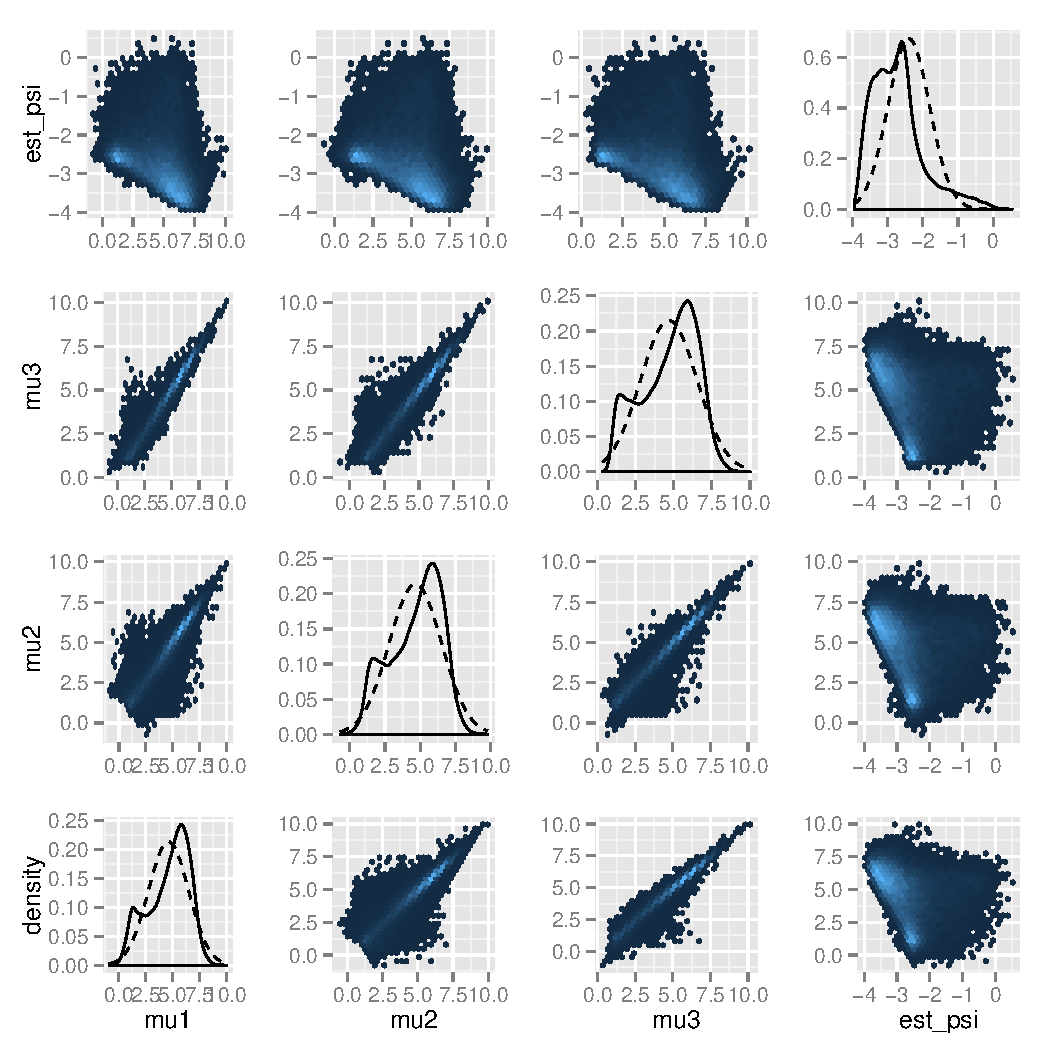
\includegraphics[width=\textwidth]{normality}}
\caption{Marginal and bivariate histograms for gene-specific parameters from a single MCMC sample, $\theta_g^{(m)}$,  for the B73 $\times$ Mo17 maize experiment. For reference, the marginal histograms have a dashed line indicating the appropriate marginal probability density functions from $N(\hat{\eta},\hat{\Sigma})$.}
\label{f:normality}
\end{figure}

Marginal and bivariate histograms for the model with an estimated covariance look similar although the estimated distribution $N(\hat{\eta},\hat{\Sigma})$ has increased variance for $\mu$ and decreased variance for $\log(\psi)$ as was previously seen in Table \ref{t:map} (results not shown). 

\section{Discussion}
\label{s:discussion}

Geneticists speculate that gene expression heterosis is one possible explanation of phenotypic
heterosis of traits, such as plant height or grain yield. Because of the unwieldy composite null hypothesis in equation \eqref{e:hypotheses}, existing methods for identifying gene expression heterosis based on RNAseq data are not directly applicable for detecting heterosis genes. \cite{ji2014estimation} introduced an empirical Bayes approach based on a hierarchical model for microarray data. We followed their approach modified slightly to allow for any number of varieties and therefore, possibly, even more complex hypotheses. We presented an empirical Bayes method to obtain MAP estimates for hyperparameters, followed by an MCMC to estimate gene-specific parameters that can be accomplished efficiently via parallelization. This methodology can be conveniently implemented in the statistical software, {\tt Stan}, which also allows for far more complex models. The empirical Bayes posteriors can be used to estimate posterior probabilities of high and low parent heterosis. 

Through a simulation study, we demonstrated that this method outperformed alternative methods (that are not designed to detect heterosis), and performed comparably well with an implementation of our model in {\tt ShrinkBayes}, which estimates the full posterior via INLA. We then demonstrated the use of the methodology on a maize experiment in which phenotypic heterosis is well known. 
% Estimates of heterosis to compare with Ji et. al.
In addition to providing estimates of heterosis probabilities and effect sizes, this real data analysis exposed violations of our normality assumptions, indicating room to improve the model and increase the power to detect gene heterosis. Some of our ongoing and future research will develop the details of such an extension.




\backmatter %  Please keep this command in your document in this position 

\section*{Acknowledgements}

The authors thank Andrew Lithio for help in implementing our model in {\tt ShrinkBayes}. Research reported in this publication was supported by National Institute of General Medical Sciences of the National Institutes of Health under award number R01GM109458. The content is solely the responsibility of the authors and does not necessarily represent the official views of the National Institutes of Health.

%  If your paper refers to supplementary web material, then you MUST
%  include this section!!  See Instructions for Authors at the journal
%  website http://www.biometrics.tibs.org

\section*{Supplementary Materials}

The supplementary materials include the maize experiment data ({\tt data.csv}), a script to run our method ({\tt script.R}), and the {\tt Stan} models: the all-genes-independent (\verb@model_ind.txt@) and covariance (\verb@model_cov.txt@) models used in obtaining MAP estimates, along with the single-gene-independent (\verb@sg_model_ind.txt@) and covariance (\verb@sg_model_cov.txt@) models used in performing the MCMC on single genes. 

\bibliography{jarad}
\bibliographystyle{biom}

% \appendix
% %  To get the journal style of heading for an appendix, mimic the following.
% \section{}
% \subsection{Material here}

\label{lastpage}

\end{document}
